\documentclass[a4paper,11pt,notitlepage,fullpage]{article}
%\documentclass{report}

\usepackage{fullpage}
\usepackage[utf8]{inputenc}
\usepackage[ngerman]{babel}
%\usepackage[english]{babel}
\usepackage{amsmath}
\usepackage{amssymb}
\usepackage{latexsym}
\usepackage{mathtools}
\usepackage{listings}
\usepackage{bbm}
%\usepackage{algorithm}
%\usepackage{algpseudocode}
\usepackage{graphicx}
\usepackage{booktabs}
\usepackage{hhline}
\usepackage{amsthm}
\usepackage{cite}
\usepackage{wrapfig}
\usepackage{hyperref}
\usepackage{titling}
\usepackage{color}

\setlength{\droptitle}{-60pt}

\newcommand{\R}{\mathbb R}
\newcommand{\p}{\mathbb P}
\newcommand{\pp}[1]{\mathbb P\left[#1\right]}
\newcommand{\E}{\mathbb E}
\newcommand{\Ee}[1]{\mathbb E\left[#1\right]}
\newcommand{\V}{\mathbb V}
\newcommand{\Vv}[1]{\mathbb V\left[#1\right]}
\newcommand{\Cov}[1]{\mathbb Cov\left[#1\right]}
\newcommand{\F}{\mathcal{F}}
\newcommand{\ind}{\mathbbm{1}}
\newcommand{\indd}[1]{\mathbbm{1}_{#1}}

\begin{document}
\author{Florian Bogner \& Alexander Palmrich}
\title{Stochastische Prozesse - Übung 6}
\maketitle

\begin{enumerate}
\setcounter{enumi}{24}

%%für ein Bild das copy-pasten und reinkommentieren
%\begin{figure}[h!]
%\centering
%\includegraphics[width=0.9\textwidth]{gfx/bildname.png}
%\label{fig1}
%\caption{TODO Beschreibung des Bildes}
%\end{figure}

%01
\item bla
\begin{enumerate}
%a
\item a
\begin{align*}
\end{align*}

%b
\item b
\begin{align*}
\end{align*}
\end{enumerate}


%02
\item bla
\begin{enumerate}
%a
\item a
\begin{align*}
\end{align*}

%b
\item b
\begin{align*}
\end{align*}
\end{enumerate}

%03
\item Wir nummerieren die Räume von 1 bis 6 zeilenweise, i.e. der Start ist 1, der Käse ist 5 und die Falle ist 6. Die Anfangsverteilung lautet $\lambda = (1,0,0,0,0,0)$ und die Übergangsmatrix lautet dann
$$P = \begin{pmatrix}
&\frac{1}{2}&\frac{1}{2}&&& \\
\frac{1}{2}&&&\frac{1}{2}&& \\
\frac{1}{3}&&&\frac{1}{3}&\frac{1}{3}& \\
&\frac{1}{3}&\frac{1}{3}&&&\frac{1}{3} \\
&&&&1& \\
&&&&&1 
\end{pmatrix}$$
In der Sprache der Markovketten sind Zustände 5 und 6 absorbierend. Die anderen Zustände sind transient. Wir suchen die Absorbtionswahrscheinlichkeit des Zustands 6 unter der gegebenen Anfangsverteilung.
Sei $p_i$ die Absorbtionswahrscheinlichkeit des Zustands 6, wenn man in Zustand $i$ startet. Offensichtlich gilt $p_5 = 0$ und $p_6 = 1$. Die anderen $p_i$ erfüllen ein Gleichungsystem. Die Absorbtionswahrscheinlichkeit ist der nach Übergangswahrscheinlichkeiten gewichtete Durchschnitt der anderen Absorbtionswahrscheinlichkeiten.
$$p_i = \sum_j P_{ij} p_j$$
Außerdem, aufgrund der Symmetrie in dem Irrgarten gilt $p_1 = 1 - p_2$ und $p_3 = 1-p_4$. Zusammengefasst und eingesetzt bekommt man die zwei Gleichungen:
\begin{align*}
p_1 &= \frac{1}{2}(1 - p_1 + p_3) \\
p_3 &= \frac{1}{3}(p_1 + 1 - p_3 + 0)
\end{align*}
Umgeformt:
\begin{align*}
3 p_1 - 1&= p_3 \\
- p_1 + 4 p_3 &= 1
\end{align*}
Erste Gleichung in zweite eingesetzt ergibt:
$$- p_1 + 4 (3 p_1 - 1) = 1$$
$$11 p_1 - 4 = 1$$
$$p_1 = \frac{5}{11}$$
Wir müssen $p_3$ gar nicht mehr berechnen, da $p_1$ gleich unsere Antwort ist: Die Maus tappt mit Wahrscheinlichtkeit $\frac{5}{11}$ in die Falle. Armes Mausi.

%04
\item bla
\begin{enumerate}
%a
\item a
\begin{align*}
\end{align*}

%b
\item b
\begin{align*}
\end{align*}
\end{enumerate}

\newpage
%05
\item Markovketten:
\begin{figure}[h!]
\centering
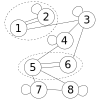
\includegraphics[width=0.5\textwidth]{gfx/29_a.pdf}
\caption{\label{fig:graph} Graph der Markovkette in 29 (a)}
\end{figure}

\begin{enumerate}
%a
\item Die Matrix lesbar aufgeschrieben lautet
\begin{align*}
P = \frac{1}{10}\begin{pmatrix}
&1&9&&&&&\\
1&9&&&&&&\\
&&6&2&&2&&\\
&&&5&5&&&\\
&&&&&4&3&3\\
&&&&10&&&\\
&&&&&&9&1\\
&&&&&&&10
\end{pmatrix}
\end{align*}
In Abbildung \ref{fig:graph} sehen wir eine graphische Representation der Markovkette. Nur positive Übergangswahrscheinlichkeiten sind eingezeichnet. Die einzige nichttriviale Kommunikationsklasse $\{1, 2\}$ ist strichliert eingezeichnet. Alle anderen Kommunikationsklassen enthalten nur einen Zustand. Damit ist die Markovkette reduzibel.
%b
\item Behauptung für $n \geq 1$:
\begin{align*}
n~\text{gerade} &\Rightarrow P^n = \begin{pmatrix}
\frac{1}{2}^n&0&\frac{1}{2}-\frac{1}{2}^n&\frac{1}{2} \\
0&\frac{1}{2}^n&\frac{1}{2}&\frac{1}{2}-\frac{1}{2}^n \\
0&0&\frac{1}{2}&\frac{1}{2}\\
0&0&\frac{1}{2}&\frac{1}{2}
\end{pmatrix} \\
n~\text{ungerade} &\Rightarrow P^n = \begin{pmatrix}
0&\frac{1}{2}^n&\frac{1}{2}&\frac{1}{2}-\frac{1}{2}^n \\
\frac{1}{2}^n&0&\frac{1}{2}-\frac{1}{2}^n&\frac{1}{2} \\
0&0&\frac{1}{2}&\frac{1}{2}\\
0&0&\frac{1}{2}&\frac{1}{2}
\end{pmatrix} 
\end{align*}

Beweis per Induktion: Induktionsanfang \emph{trivial}.

Gerader Induktionsschritt:
\begin{gather*}
P^n = P^{n-1} \cdot P = \begin{pmatrix}
0&\frac{1}{2}^{n-1}&\frac{1}{2}&\frac{1}{2}-\frac{1}{2}^{n-1} \\
\frac{1}{2}^{n-1}&0&\frac{1}{2}-\frac{1}{2}^{n-1}&\frac{1}{2} \\
0&0&\frac{1}{2}&\frac{1}{2}\\
0&0&\frac{1}{2}&\frac{1}{2}
\end{pmatrix} \cdot \begin{pmatrix}
0&\frac{1}{2}&\frac{1}{2}&0 \\
\frac{1}{2}&0&0&\frac{1}{2} \\
0&0&\frac{1}{2}&\frac{1}{2}\\
0&0&\frac{1}{2}&\frac{1}{2}
\end{pmatrix} \\
= \begin{pmatrix}
\frac{1}{2}^{n-1} \cdot \frac{1}{2} & 0 & \frac{1}{2}\cdot\frac{1}{2} + (\frac{1}{2} - \frac{1}{2}^{n-1})\cdot\frac{1}{2} & \frac{1}{2}^{n-1} \cdot \frac{1}{2} + \frac{1}{2}\cdot\frac{1}{2} +  (\frac{1}{2} - \frac{1}{2}^{n-1})\cdot\frac{1}{2}\\
0 & \frac{1}{2}^{n-1} \cdot \frac{1}{2} & \frac{1}{2}^{n-1} \cdot \frac{1}{2} + \frac{1}{2}\cdot\frac{1}{2} +  (\frac{1}{2} - \frac{1}{2}^{n-1})\cdot\frac{1}{2} & \frac{1}{2}\cdot\frac{1}{2} + (\frac{1}{2} - \frac{1}{2}^{n-1})\cdot\frac{1}{2} \\
0&0&\frac{1}{2}\cdot\frac{1}{2} + \frac{1}{2}\cdot\frac{1}{2}&\frac{1}{2}\cdot\frac{1}{2} + \frac{1}{2}\cdot\frac{1}{2}\\
0&0&\frac{1}{2}\cdot\frac{1}{2} + \frac{1}{2}\cdot\frac{1}{2}&\frac{1}{2}\cdot\frac{1}{2} + \frac{1}{2}\cdot\frac{1}{2}
\end{pmatrix} \\
= \begin{pmatrix}
\frac{1}{2}^n&0&\frac{1}{2}-\frac{1}{2}^n&\frac{1}{2} \\
0&\frac{1}{2}^n&\frac{1}{2}&\frac{1}{2}-\frac{1}{2}^n \\
0&0&\frac{1}{2}&\frac{1}{2}\\
0&0&\frac{1}{2}&\frac{1}{2}
\end{pmatrix}
\end{gather*}

Ungerader Induktionsschritt analog:
\begin{gather*}
P^n = P^{n-1} \cdot P = \begin{pmatrix}
\frac{1}{2}^{n-1}&0&\frac{1}{2}-\frac{1}{2}^{n-1}&\frac{1}{2} \\
0&\frac{1}{2}^{n-1}&\frac{1}{2}&\frac{1}{2}-\frac{1}{2}^{n-1} \\
0&0&\frac{1}{2}&\frac{1}{2}\\
0&0&\frac{1}{2}&\frac{1}{2}
\end{pmatrix} \cdot \begin{pmatrix}
0&\frac{1}{2}&\frac{1}{2}&0 \\
\frac{1}{2}&0&0&\frac{1}{2} \\
0&0&\frac{1}{2}&\frac{1}{2}\\
0&0&\frac{1}{2}&\frac{1}{2}
\end{pmatrix} \\
= \begin{pmatrix}
0 & \frac{1}{2}^{n-1} \cdot \frac{1}{2} & \frac{1}{2}^{n-1} \cdot \frac{1}{2} + \frac{1}{2}\cdot\frac{1}{2} +  (\frac{1}{2} - \frac{1}{2}^{n-1})\cdot\frac{1}{2} & \frac{1}{2}\cdot\frac{1}{2} + (\frac{1}{2} - \frac{1}{2}^{n-1})\cdot\frac{1}{2} \\
\frac{1}{2}^{n-1} \cdot \frac{1}{2} & 0 & \frac{1}{2}\cdot\frac{1}{2} + (\frac{1}{2} - \frac{1}{2}^{n-1})\cdot\frac{1}{2} & \frac{1}{2}^{n-1} \cdot \frac{1}{2} + \frac{1}{2}\cdot\frac{1}{2} +  (\frac{1}{2} - \frac{1}{2}^{n-1})\cdot\frac{1}{2}\\
0&0&\frac{1}{2}\cdot\frac{1}{2} + \frac{1}{2}\cdot\frac{1}{2}&\frac{1}{2}\cdot\frac{1}{2} + \frac{1}{2}\cdot\frac{1}{2}\\
0&0&\frac{1}{2}\cdot\frac{1}{2} + \frac{1}{2}\cdot\frac{1}{2}&\frac{1}{2}\cdot\frac{1}{2} + \frac{1}{2}\cdot\frac{1}{2}
\end{pmatrix} \\
= \begin{pmatrix}
0&\frac{1}{2}^n&\frac{1}{2}&\frac{1}{2}-\frac{1}{2}^n \\
\frac{1}{2}^n&0&\frac{1}{2}-\frac{1}{2}^n&\frac{1}{2} \\
0&0&\frac{1}{2}&\frac{1}{2}\\
0&0&\frac{1}{2}&\frac{1}{2}
\end{pmatrix}
\end{gather*}
\qed

Im Grenzwert:
\begin{align*}
P^\infty = \begin{pmatrix}
0&0&\frac{1}{2}&\frac{1}{2}\\
0&0&\frac{1}{2}&\frac{1}{2}\\
0&0&\frac{1}{2}&\frac{1}{2}\\
0&0&\frac{1}{2}&\frac{1}{2}
\end{pmatrix}
\end{align*}

Daraus sieht man die Zustände 1 und 2 sind gemeinsam in einer Kommunikationsklasse transient und analog sind die Zustände 3 und 4 in einer Kommunikationsklasse rekurrent.
\end{enumerate}

\end{enumerate}



\end{document}
